\chapter{Derivation of Stream Equations}\doublelabel{derivation-of-stream-equations}

This appendix contains a derivation of the equation for stream
connectors from \autoref{stream-connectors}.

\section{Reasons for avoiding the actual mixing enthalpy in connector definitions}\doublelabel{reasons-for-avoiding-the-actual-mixing-enthalpy-in-connector-definitions}

Consider a connection set with \emph{n} connectors. The mixing enthalpy
is defined by the mass balance
\begin{equation*}
0=\sum_{j=1}^n\dot{m}_j
\end{equation*}
and the energy balance
\begin{equation*}
0=\sum_{j=1}^n\dot{H}_j
\end{equation*}
with
\begin{equation*}
\dot{H}_j=\dot{m}_j
\begin{cases}
h_{mix}&\text{if $\dot{m}_j>0$}\\
h_{outflow,j}&\text{if $\dot{m}_j<=0$}
\end{cases}
\end{equation*}
Herein, mass flow rates are positive when entering models (exiting the
connection set). The specific enthalpy represents the specific enthalpy
inside the component, close to the connector, for the case of outflow.
Expressed with variables used in the balance equations we arrive at:
\begin{equation*}
h_{outflow,j}=
\begin{cases}
\frac{\dot{H}_j}{\dot{m}_j}&\text{if $\dot{m}_j<0$}\\
\textrm{arbitrary}&\text{if $\dot{m}_j>=0$}
\end{cases}
\end{equation*}
While these equations are suitable for device-oriented modeling, the
straightforward usage of this definition leads to models with
discontinuous residual equations, which violates the prerequisites of
several solvers for nonlinear equation systems. This is the reason why
the actual mixing enthalpy is not modelled directly in the model
equations. The stream connectors provide a suitable alternative.

\begin{figure}[H]
\caption{Exemplary connection set with three connected components and a common mixing enthalpy}
\begin{center}
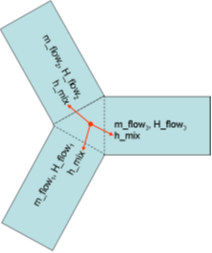
\includegraphics[width=3in,height=3in]{fluidmix}
\end{center}
\end{figure}

\section{Rationale for the formulation of the inStream() operator}\doublelabel{rationale-for-the-formulation-of-the-instream-operator}

For simplicity, the derivation of the inStream() operator is shown at
hand of 3 model components that are connected together. The case for N
connections follows correspondingly.

The energy and mass balance equations for the connection set for 3
components are (see above):
\begin{subequations}
\begin{equation}
\begin{split}
0=&\dot{m}_1\cdot
\begin{cases}
h_{mix}&\text{if $\dot{m}_1>0$}\\
h_{outflow,1}&\text{if $\dot{m}_1<=0$}
\end{cases}\\
+&\dot{m}_2\cdot
\begin{cases}
h_{mix}&\text{if $\dot{m}_2>0$}\\
h_{outflow,2}&\text{if $\dot{m}_2<=0$}
\end{cases}\\
+&\dot{m}_3\cdot
\begin{cases}
h_{mix}&\text{if $\dot{m}_3>0$}\\
h_{outflow,3}&\text{if $\dot{m}_3<=0$}
\end{cases}
\end{split}
\label{eq:D1a}
\end{equation}
\begin{equation}
0=\dot{m}_1+\dot{m}_2+\dot{m}_3
\label{eq:D1b}
\end{equation}
\label{eq:D1}
\end{subequations}

The balance equations are implemented using a max() operator in place of
the piecewise expressions, taking care of the different flow directions:
\begin{subequations}
\begin{equation}
\begin{split}
0=&\text{max}(\dot{m}_1,0)h_{mix}-\text{max}(-\dot{m}_1,0)h_{outflow,1}\\
+&\text{max}(\dot{m}_2,0)h_{mix}-\text{max}(-\dot{m}_2,0)h_{outflow,2}\\
+&\text{max}(\dot{m}_3,0)h_{mix}-\text{max}(-\dot{m}_3,0)h_{outflow,3}
\end{split}
\label{eq:D2a}
\end{equation}

\begin{equation}
\begin{split}
0=&\text{max}(\dot{m}_1,0)-\text{max}(-\dot{m}_1,0)\\
+&\text{max}(\dot{m}_2,0)-\text{max}(-\dot{m}_2,0)\\
+&\text{max}(\dot{m}_3,0)-\text{max}(-\dot{m}_3,0)
\end{split}
\label{eq:D2b}
\end{equation}
\label{eq:D2}
\end{subequations}

Equation (\ref{eq:D2a}) is solved for $h_{mix}$
\begin{equation*}
h_{mix}=\frac{\text{max}(-\dot{m}_1,0)h_{outflow,1}+\text{max}(-\dot{m}_2,0)h_{outflow,2}+\text{max}(-\dot{m}_3,0)h_{outflow,3}}
{\text{max}(\dot{m}_1,0)+\text{max}(\dot{m}_2,0)+\text{max}(\dot{m}_3,0)}
\end{equation*}
Using (\ref{eq:D2b}), the denominator can be changed to:
\begin{equation*}
h_{mix}=\frac{\text{max}(-\dot{m}_1,0)h_{outflow,1}+\text{max}(-\dot{m}_2,0)h_{outflow,2}+\text{max}(-\dot{m}_3,0)h_{outflow,3}}
{\text{max}(-\dot{m}_1,0)+\text{max}(-\dot{m}_2,0)+\text{max}(-\dot{m}_3,0)}
\end{equation*}
Above it was shown that an equation of this type does not yield properly
formulated model equations. In the streams concept we therefore decide
to split the energy balance, which consists of different branches
depending on the mass flow direction. Consequently, separate energy
balances are the result; each valid for specific flow directions.

In a model governing equations have to establish the specific enthalpy
of fluid leaving the model based on the specific enthalpy of fluid
flowing into it. Whenever the mixing enthalpy is \emph{used} in a model
it is therefore the mixing enthalpy under the assumption of fluid
flowing into said model.

We establish this quantity using a dedicated operator $inStream(h_{outflow,i})=h_{mix}$ assuming that $\dot{m}_{i} >= 0$. This leads to
three different incarnations of (n in the general case). This is
illustrated in the figure below. For the present example of three
components in a connection set, this means the following.
\begin{eqnarray*}
inStream(h_{outflow,1})&=&\frac{\text{max}(-\dot{m}_2,0)h_{outflow,2}+\text{max}(-\dot{m}_3,0)h_{outflow,3}}{\text{max}(-\dot{m}_2,0)+\text{max}(-\dot{m}_3,0)}\\
inStream(h_{outflow,2})&=&\frac{\text{max}(-\dot{m}_1,0)h_{outflow,1}+\text{max}(-\dot{m}_3,0)h_{outflow,3}}{\text{max}(-\dot{m}_1,0)+\text{max}(-\dot{m}_3,0)}\\
inStream(h_{outflow,3})&=&\frac{\text{max}(-\dot{m}_1,0)h_{outflow,1}+\text{max}(-\dot{m}_2,0)h_{outflow,2}}{\text{max}(-\dot{m}_1,0)+\text{max}(-\dot{m}_2,0)}
\end{eqnarray*}
\begin{figure}[H]
\caption{Exemplary connection set with three connected components}
\begin{center}
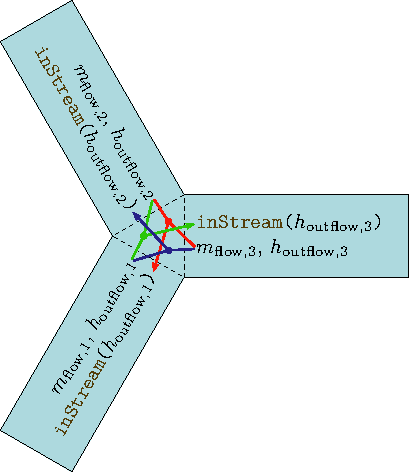
\includegraphics[width=3in,height=3in]{fluidmix3}
\end{center}
\end{figure}

In the general case of a connection set with \emph{n} components,
similar considerations lead to the following.
\begin{equation*}
inStream(h_{outflow,i})=\frac{\sum_{j=1,...,n;j\neq i}\text{max}(-\dot{m}_j,0)h_{outflow,j}}{\sum_{j=1,...,n;j\neq i}\text{max}(-\dot{m}_j,0)}
\end{equation*}

\section{Special cases covered by the inStream() operator definition}\doublelabel{special-cases-covered-by-the-instream-operator-definition}
\subsection{Stream connector is not connected (N=1):}\doublelabel{stream-connector-is-not-connected-n-1}
For this case, the return value of the \lstinline!inStream()! operator is arbitrary.
Therefore, it is set to the outflow value.

\subsection{Connection of 2 stream connectors, one to one connections (N=2):}\doublelabel{connection-of-2-stream-connectors-one-to-one-connections-n-2}

\begin{eqnarray*}
inStream(h_{outflow,1})&=&\frac{\text{max}(-\dot{m}_2,0)h_{outflow,2}}{\text{max}(-\dot{m}_2,0)}=h_{outflow,2}\\
inStream(h_{outflow,2})&=&\frac{\text{max}(-\dot{m}_1,0)h_{outflow,1}}{\text{max}(-\dot{m}_1,0)}=h_{outflow,1}
\end{eqnarray*}

In this case, \lstinline!inStream()! is continuous (contrary to $h_{mix}$) and does not
depend on flow rates. The latter result means that this transformation
may remove nonlinear systems of equations, which requires that either
simplifications of the form ``a*b/a = b'' must be provided, or that this
case is treated directly.

\subsection{Connection of 3 stream connectors where one mass flow rate is identical to zero (N=3 and $\dot{m}_3=0$):}\doublelabel{connection-of-3-stream-connectors-where-one-mass-flow-rate-is-identical-to-zero-n-3-and}
This case occurs, when a one-port sensor (like a temperature sensor) is
connected to two connected components. For the sensor, the min attribute
of the mass flow rate should be set to zero (no fluid exiting the
component via this connector).
This simplification (and similar ones) can also be used if a tool determines that a mass flow rate is zero or non-negative.
It is also possible to generalize this to the case where more than one sensor is connected.
The suggested implementation results in
the following equations, and as indicated the last formula can be
simplified further by using $\dot{m}_3=0$:
\begin{eqnarray*}
inStream(h_{outflow,1})&=&h_{outflow,2}\\
inStream(h_{outflow,2})&=&h_{outflow,1}\\
inStream(h_{outflow,3})&=&\frac{\text{max}(-\dot{m}_1,0)h_{outflow,1}+\text{max}(-\dot{m}_2,0)h_{outflow,2}}{\text{max}(-\dot{m}_1,0)+\text{max}(-\dot{m}_2,0)}\\
&=&\begin{cases}
h_{outflow,2}&\text{if $\dot{m}_1>=0$}\\
h_{outflow,1}&\text{if $\dot{m}_1<0$ and $\dot{m}_3=0$}
\end{cases}
\end{eqnarray*}
\begin{figure}[H]
\caption{Example series connection of multiple models with stream connectors }
\begin{center}
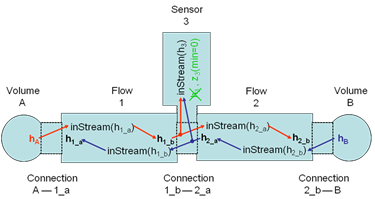
\includegraphics[width=6in,height=3in]{fluidmix4}
\end{center}
\end{figure}

For the two components with finite mass flow rates (not the sensor), the
properties discussed for two connected components still hold. The
connection set equations reflect that the sensor does not any influence
by discarding the flow rate of the latter. In several cases a non-linear
equation system is removed by this transformation. However, \lstinline!inStream(..)!
results in a discontinuous equation for the sensor, which is consistent
with modeling the convective phenomena only. The discontinuous equation
is uncritical, if the sensor variable is not used in a feedback loop
with direct feedthrough, since the discontinuous equation is then not
part of an algebraic loop. Otherwise, it is advisable to regularize or
filter the sensor signal.

\subsection{Connection of 3 stream connectors where two mass flow rates are positive (ideal splitting junction for uni-directional flow)}\doublelabel{connection-of-3-stream-connectors-where-two-mass-flow-rates-are-positive-ideal-splitting-junction-for-uni-directional-flow}

If uni-directional flow is present and an ideal splitter is modelled,
the required flow direction should be defined in the connector instance
with the ``\lstinline!min!'' attribute (the ``\lstinline!max!'' attribute could be also defined,
however it does not lead to simplifications):

\begin{lstlisting}[language=modelica]
model m2
  Fluidport c(m_flow(min=0));
  ...
end m2;
\end{lstlisting}

Consider the case of and all other mass flow rates positive (with the
min attribute set accordingly). Connecting \lstinline!m1.c! with \lstinline!m2.c! and \lstinline!m3.c!, such
that

\begin{lstlisting}[language=modelica]
  m2.c.m_flow.min = 0; // max(-m2.c.m_flow,0) = 0
  m3.c.m_flow.min = 0; // max(-m3.c.m_flow,0) = 0
\end{lstlisting}
results in the following equation:
\begin{equation*}
inStream(h_{outflow,1})=\frac{\text{max}(-\dot{m}_2,0)h_{outflow,2}+\text{max}(-\dot{m}_3,0)h_{outflow,3}}{\text{max}(-\dot{m}_2,0)+\text{max}(-\dot{m}_3,0)}=\frac{0}{0}
\end{equation*}

The \lstinline!inStream()! operator cannot be evaluated for a connector, on which
the mass flow rate has to be negative by definition. The reason is that
the value is arbitrary, which is why it is defined as follows.
\begin{equation*}
inStream(h_{outflow,1}):=h_{outflow,1}
\end{equation*}
For the remaining connectors the inStream() operator reduces to a simple
result.
\begin{eqnarray*}
inStream(h_{outflow,2})&=\frac{\text{max}(-\dot{m}_1,0)h_{outflow,1}+\text{max}(-\dot{m}_3,0)h_{outflow,3}}{\text{max}(-\dot{m}_1,0)+\text{max}(-\dot{m}_3,0)}=h_{outflow,1}\\
inStream(h_{outflow,3})&=\frac{\text{max}(-\dot{m}_1,0)h_{outflow,1}+\text{max}(-\dot{m}_2,0)h_{outflow,2}}{\text{max}(-\dot{m}_1,0)+\text{max}(-\dot{m}_2,0)}=h_{outflow,1}
\end{eqnarray*}
Again, the previous non-linear algebraic system of equations is removed.
This means that utilizing the information about uni-directional flow is
very important.

To summarize, if all mass flow rates are zero, the balance equations for
stream variables (\ref{eq:D1}) and for flows (\ref{eq:D2}) are identically fulfilled. In
such a case, any value of h\_mix fulfills (\ref{eq:D1}), i.e., a unique
mathematical solution does not exist. This specification only requires
that a solution fulfills the balance equations. Additionally, a
recommendation is given to compute all unknowns in a unique way, by
providing an explicit formula for the \lstinline!inStream! operator. Due to the
definition, that only flows where the corresponding ``min'' attribute is
neither zero nor positive enter this formula, a meaningful physcial
result is always obtained, even in case of zero mass flow rate. As a
side effect, non-linear equation systems are automatically removed in
special cases, like sensors or uni-directional flow, without any
symbolic transformations (no equation must be analyzed; only the
``\lstinline!min!''-attributes of the corresponding flow variables).
